
\documentclass[letterpaper]{article}

\usepackage[margin=3.2cm]{geometry}
\usepackage{amsmath}
\usepackage{amsfonts}
\usepackage{txfonts}
\usepackage{multirow}
\usepackage{tikz} \usetikzlibrary{arrows.meta,patterns}
\usepackage{hyperref}
\hypersetup{colorlinks,linkcolor=blue,citecolor=blue,urlcolor=blue}
\urlstyle{same}

\renewcommand{\arraystretch}{1.2}

\newcommand{\vect}[1]{\mathbf#1}
\newcommand{\vecp}[1]{\tilde{\mathbf#1}}
\newcommand{\nab}{\vect{\nabla}}
\newcommand{\keyw}[1]{\texttt{\small #1}}


\begin{document}

\thispagestyle{empty}
\begin{center}

\vspace*{1in}
{
\Large Formulations for the finite element method\\\vspace{6pt}
and the GetDP software}

\vspace*{0.3in}
{Marc Boul\'e} 

\url{marc.boule@etsmtl.ca}

\vspace*{0.1in}
\today

\end{center}

This document is a work in progress aiming to show a set of formulations based on the Laplace/Poisson equations for use in the finite element method. Implementation notes for the GetDP software are also briefly given. Electromagnetic notation mostly follows the textbook ``\textit{Introduction to electrodynamics}'' by D. J. Griffiths. The symbol ${i}$ is the imaginary unit. When required, scalar phasors are denoted $\tilde{A}$, with $A(t)=\text{Re}[\tilde{A}e^{i\omega t}]$ and vector phasors are denoted $\vecp{A}$, with $\vect{A}(t)=\text{Re}[\vecp{A}e^{i\omega t}]$.

The simulation domain is denoted $\Omega$, and its boundary is denoted $\Gamma$. The Neumann-type portion of the domain's boundary, if required, is denoted $\Gamma_N$. The Dirichlet-type portion of the domain's boundary, if required, is denoted $\Gamma_D$. 
Each can be subdivided into multiple disjoint subregions, but are treated as a single type for the sake of simplicity. 
% and is assumed to be implicit in all formulations (the unknown or its normal component is explicitly imposed on the Dirichlet boundary). 
Thus, $\Gamma=\Gamma_D\cup\Gamma_N$.

All weighting functions (sometimes called test functions) are denoted $W$ or $\vect{W}$. In the numerical implementation, it is assumed that $W=0$ or $\vect{n}\times\vect{W}=\vect{0}$ on $\Gamma_D$. The unit vector $\vect{n}$ is normal to $\Gamma$ and points outward. All material parameters such as permittivity, permeability, electric or thermal conductivity, are assumed to be scalar values.

The following formulations appear in this document:

\begin{tabular}{l}
\hyperlink{sec_gsp}{\ref{sec_gsp}~\nameref{sec_gsp}} \\
\hyperlink{sec_esp}{\ref{sec_esp}~\nameref{sec_esp}} \\
\hyperlink{sec_msp}{\ref{sec_msp}~\nameref{sec_msp}} \\
\hyperlink{sec_mvp}{\ref{sec_mvp}~\nameref{sec_mvp}} \\
\hyperlink{sec_ksp}{\ref{sec_ksp}~\nameref{sec_ksp}} \\
\hyperlink{sec_tsp}{\ref{sec_tsp}~\nameref{sec_tsp}} \\
\hyperlink{sec_fsp}{\ref{sec_fsp}~\nameref{sec_fsp}} \\
\hyperlink{sec_mqs}{\ref{sec_mqs}~\nameref{sec_mqs}} \\
\end{tabular}





%------------------------------------------------------------------------------
\clearpage
\section{Newtonian gravitation -- Scalar potential}
\label{sec_gsp}
%------------------------------------------------------------------------------

\hypertarget{sec_gsp}{Simple} gravitation not involving general relativity.

\begin{table}[h!]
\centering
\begin{tabular}{lll}
\hline
\multicolumn{3}{c}{Governing law:} \\
\multicolumn{3}{c}{$\nab\cdot\vect{g}=-4\pi G\rho$}\\
$\vect{g}=-\nab V$ & $[\text{N}\cdot \text{kg}^{-1}%=\text{m}\cdot \text{s}^{-2}
]$ & Gravitational field (gravitational acceleration)\\
$V$ & $[%\text{J}\cdot \text{kg}^{-1}=
\text{N}\cdot \text{m}\cdot \text{kg}^{-1}]$ & Gravitational potential ($V\leq0$)\\
$G$ & $[\text{N}\cdot\text{m}^{2}\cdot\text{kg}^{-2}]$ & Universal gravitational constant\\
$\rho$ & $[\text{kg}\cdot \text{m}^{-3}]$ & Mass density\\

\hline

\multicolumn{3}{c}{Strong form:} \\
\multicolumn{3}{c}{$\nab\cdot\left(\nab V\right)=4\pi G\rho$}\\
\hline

\multicolumn{3}{c}{Weak form:} \\[1pt]
\multicolumn{3}{c}{$\displaystyle\int_\Omega \nab V\cdot\nab W\,d\Omega+
\int_{\Gamma_N}\vect{n}\cdot\vect{g}\,W\,d{\Gamma_N}+
4\pi G\int_\Omega \rho\,W\,d\Omega=0$}\\[8pt]
 $V=0$ & \multicolumn{2}{l}{on $\Gamma_D$, homogeneous Dirichlet (normal $\vect{g}$)}\\
$\vect{n}\cdot\vect{g}=0$ & \multicolumn{2}{l}{on $\Gamma_N$, homogeneous Neumann (tangent $\vect{g}$)}\\
$\vect{n}\cdot\vect{g}=g_{n,N}(\vect{r})$ & \multicolumn{2}{l}{on $\Gamma_N$, nonhomogeneous Neumann (normal component of gravitational}\\
 & \multicolumn{2}{l}{field, positive when field exits $\Omega$, negative when field enters $\Omega$)}\\
 $\vect{n}\cdot\vect{g}=V/R$ & \multicolumn{2}{l}{on $\Gamma_N$, first order asymptotic boundary condition (3D/axisym.)}\\

\hline
\multicolumn{3}{c}{Post-processing:} \\
$W_{g}=\frac{-1}{8\pi G}\!\int g^2\,d\Omega$ & $[\text{J}]$ & Gravitational energy\\[1pt]

%$\vect{F}\cdot\vect{n}=mkT/R$ & \multicolumn{2}{l}{on $\Gamma_N$, first order asymptotic boundary condition ($m$ is harmonic \#)}\\
\hline
\end{tabular}
\end{table}

%The correspondance between the electrostatic scalar formulation (without permanent polarization) and the themal conduction scalar formulation is  
%\begin{equation}
%V\leftrightarrow V\qquad\quad
%\varepsilon_0\leftrightarrow 1 \qquad\quad
%\rho\leftrightarrow -4\pi G\rho\qquad\quad
%\vect{E}\leftrightarrow\vect{g}\qquad\quad
%\end{equation}









%------------------------------------------------------------------------------
\clearpage
\section{Electrostatics -- Scalar potential}
\label{sec_esp}
%------------------------------------------------------------------------------

\hypertarget{sec_esp}{Permanent} polarization $\vect{P}_p$ is included but can be set to $\vect{0}$ when not needed.

\begin{table}[h!]
\centering
\begin{tabular}{lll}
\hline
\multicolumn{3}{c}{Governing law:} \\
\multicolumn{3}{c}{$\nab\cdot\vect{D}=\rho$}\\
$\vect{D}$ & $[\text{C}\cdot \text{m}^{-2}]$ & Electric displacement field\\
$\rho$ & $[\text{C}\cdot \text{m}^{-3}]$ & Free charge density\\
\hline

\multicolumn{3}{c}{Constitutive relation:} \\
\multicolumn{3}{c}{ $\vect{D}=\varepsilon\vect{E}+\vect{P}_{p}$}\\
$\varepsilon=\varepsilon_r\varepsilon_0$ & $[\text{C}^2 \cdot \text{N}^{-1} \cdot \text{m}^{-2}]$ & Electric permittivity of medium\\ %\multirow{2}{*}{}
$\varepsilon_0$ &  $[\text{C}^2 \cdot \text{N}^{-1} \cdot \text{m}^{-2}]$ & Vacuum permittivity\\
$\varepsilon_r$ & $[1]$ & Relative permittivity of medium\\
$\vect{E}=-\nab V$ & $[\text{V}\cdot \text{m}^{-1}]$ & Electric field\\
$V$ & $[\text{V}]$ & Electric potential\\
$\vect{P}_p$ & $[\text{C}\cdot \text{m}^{-2}]$ & Permanent polarization of medium\\
\hline

\multicolumn{3}{c}{Strong form:} \\[1pt]
\multicolumn{3}{c}{$-\nab\cdot\left(\varepsilon\nab V+\vect{P}_{p}\right)=\rho$}\\[3pt]
\hline

\multicolumn{3}{c}{Weak form:} \\[1pt]
\multicolumn{3}{c}{$\displaystyle\int_\Omega\varepsilon\nab V\cdot\nab W\,d\Omega
-\int_\Omega\vect{P}_p\cdot\nab W\,d\Omega
+\int_{\Gamma_N}\vect{n}\cdot\vect{D}\,W\,d{\Gamma_N}
-\int_\Omega\rho\,W\,d\Omega=0$}\\[8pt]
$V=V_D$ & \multicolumn{2}{l}{on $\Gamma_D$, constant Dirichlet (normal $\vect{E}$; normal $\vect{D}$ when normal $\vect{P}_p$); charge $Q$ $[\text{C}]$}\\
 & \multicolumn{2}{l}{is the associated (dual) global quantity for a floating potential}\\
$V=V_D(\vect{r})$ & \multicolumn{2}{l}{on $\Gamma_D$, nonhomogeneous Dirichlet (general case)}\\
$\vect{n}\cdot\vect{D}=0$ & \multicolumn{2}{l}{on $\Gamma_N$, homogeneous Neumann (tangent $\vect{D}$; tangent $\vect{E}$ when tangent $\vect{P}_p$)}\\
$\vect{n}\cdot\vect{D}=-\sigma_N(\vect{r})$ & \multicolumn{2}{l}{on $\Gamma_N$, nonhomogeneous Neumann (prescribed surface charge density)}\\
$\vect{n}\cdot\vect{D}=m\varepsilon_0V/R$ & \multicolumn{2}{l}{on $\Gamma_N$, first order asymptotic boundary condition, $m=1$ for 2D planar without net}\\
 & \multicolumn{2}{l}{charge or 3D/axisym. with net charge, $m=2$ for 3D/axisym. without net charge }\\
 
\hline
\multicolumn{3}{c}{Post-processing:} \\
$W_E=\frac{1}{2}\!\int\varepsilon E^2\,d\Omega$ & $[\text{J}]$ & Electrostatic energy\\[1pt]
$W_D=\frac{1}{2}\!\int\frac{1}{\varepsilon} D^2\,d\Omega$ & $[\text{J}]$ & Electrostatic coenergy (equal to energy when $\vect{P}_{p}=\vect{0}$)\\[1pt]

 
\hline
\end{tabular}
\end{table}
% to go from strong to weak, start with div(D) on left side
% apply product rule (5) from Griffiths, two integrals will result
% for grad(W).D, apply constitutive relation and write as two integrals (the first two in weak)
% for div(W*D), apply divergence theorem then rearrange, (resulting in third integral in weak)
% last term is direct inegral of product of W with rho

% for normal and tangent remarks, see Zhu 2006 eqs. (3.5, 3.6)
% for negative sign in nonhomogeneous Neumann, see Sabine Zaglmayr PhD thesis eq. (2.16)





%------------------------------------------------------------------------------
\clearpage
\section{Magnetostatics -- Scalar potential}
\label{sec_msp}
%------------------------------------------------------------------------------

\hypertarget{sec_msp}{This} formulation is applicable when no free currents exist. Permanent magnetization $\vect{M}_p$ is included but can be set to $\vect{0}$ when not needed. 
The quantity $\mu_0\vect{M}_{p}$ represents the remanent magnetic field in the magnet (called $\vect{B}_r$). Linear permanent magnets are sometimes specified by their coercive $\vect{H}$ field instead (called $\vect{H}_c$). The equalities below can be invoked as needed:
\begin{equation}
\label{eqMBrHc}
\mu_0\vect{M}_{p}=\vect{B}_r=\mu\vect{H}_c
\end{equation}

\begin{table}[h!]
\centering
\begin{tabular}{lll}
\hline
\multicolumn{3}{c}{Governing law:} \\
\multicolumn{3}{c}{$\nab\cdot\vect{B}=0$}\\
$\vect{B}$ & $[\text{T}]$ & Magnetic field\\
\hline

\multicolumn{3}{c}{Constitutive relation:} \\
\multicolumn{3}{c}{ $\vect{B}=\mu\vect{H}+\mu_0\vect{M}_{p}$}\\
$\mu=\mu_r\mu_0$ & $[\text{T} \cdot \text{m} \cdot \text{A}^{-1}]$ & Magnetic permeability of medium\\ %\multirow{2}{*}{}
$\mu_0$ &  $[\text{T} \cdot \text{m} \cdot \text{A}^{-1}]$ & Vacuum permeability\\
$\mu_r$ & $[1]$ & Relative permeability of medium\\
$\vect{H}=-\nab \varphi$ & $[\text{A}\cdot \text{m}^{-1}]$ & Auxiliary field\\
$\varphi$ & $[\text{A}]$ & Magnetic scalar potential\\
$\vect{M}_p$ & $[\text{A}\cdot \text{m}^{-1}]$ & Permanent magnetization of medium\\
\hline

\multicolumn{3}{c}{Strong form:} \\[1pt]
\multicolumn{3}{c}{$-\nab\cdot\left(\mu\nab \varphi+\mu_0\vect{M}_{p}\right)=0$}\\[3pt]
\hline

\multicolumn{3}{c}{Weak form:} \\[1pt]
\multicolumn{3}{c}{$\displaystyle\int_\Omega\mu\nab \varphi\cdot\nab W\,d\Omega
-\int_\Omega\mu_0\vect{M}_p\cdot\nab W\,d\Omega
+\int_{\Gamma_N}\vect{n}\cdot\vect{B}\,W\,d{\Gamma_N}
=0$}\\[8pt]
$\varphi=\varphi_D$ & \multicolumn{2}{l}{on $\Gamma_D$, constant Dirichlet (normal $\vect{H}$; normal $\vect{B}$ when normal $\vect{M}_p$)}\\
$\varphi=\varphi_D(\vect{r})$ & \multicolumn{2}{l}{on $\Gamma_D$, nonhomogeneous Dirichlet (general case)}\\
$\vect{n}\cdot\vect{B}=0$ & \multicolumn{2}{l}{on $\Gamma_N$, homogeneous Neumann (tangent $\vect{B}$; tangent $\vect{H}$ when tangent $\vect{M}_p$)}\\
$\vect{n}\cdot\vect{B}=-\sigma_{N}(\vect{r})$ & \multicolumn{2}{l}{on $\Gamma_N$, nonhomogeneous Neumann (fictitious magnetic surface charge density)}\\
$\vect{n}\cdot\vect{B}=m\mu_0\varphi/R$ & \multicolumn{2}{l}{on $\Gamma_N$, first order asymptotic boundary condition, $m=1$ for 2D planar, $m=2$}\\
 & \multicolumn{2}{l}{for 3D/axisymmetric (no net magnetic charge, i.e. no magnetic monopoles)}\\
 
\hline
\multicolumn{3}{c}{Post-processing:} \\
$W_H=\frac{1}{2}\!\int\mu H^2\,d\Omega$ & $[\text{J}]$ & Magnetostatic energy\\[1pt]
$W_B=\frac{1}{2}\!\int\frac{1}{\mu} B^2\,d\Omega$ & $[\text{J}]$ & Magnetostatic coenergy (equal to energy when $\vect{M}_{p}=\vect{0}$)\\[1pt]


 
\hline
\end{tabular}
\end{table}

The correspondance between the electrostatic scalar formulation (without free charges) and the magnetostatic scalar formulation is  
\begin{equation}
\vect{D}\leftrightarrow\vect{B}\qquad\quad
\vect{E}\leftrightarrow\vect{H}\qquad\quad
\vect{P}_{\!p}\leftrightarrow\mu_0\vect{M}_{p}\qquad\quad
\varepsilon_0\leftrightarrow\mu_0\qquad\quad
\varepsilon_r\leftrightarrow\mu_r\qquad\quad
\varepsilon\leftrightarrow\mu
\end{equation}





%------------------------------------------------------------------------------
\clearpage
\section{Magnetostatics -- Vector potential}
\label{sec_mvp}
%------------------------------------------------------------------------------

\hypertarget{sec_mvp}{This} formulation is required when free currents exist. Permanent magnetization $\vect{M}_p$ is included but can be set to $\vect{0}$ when not needed. 
The quantity $\mu_0\vect{M}_{p}$ represents the remanent magnetic field in the magnet (called $\vect{B}_r$). Linear permanent magnets are sometimes specified by their coercive $\vect{H}$ field instead (called $\vect{H}_c$). The equalities below can be invoked as needed:
\begin{equation}
\label{eqMBrHc2}
\mu_0\vect{M}_{p}=\vect{B}_r=\mu\vect{H}_c
\end{equation}

\begin{table}[h!]
\centering
\begin{tabular}{lll}
\hline
\multicolumn{3}{c}{Governing law:} \\
\multicolumn{3}{c}{$\nab\times\vect{H}=\vect{J}$}\\
$\vect{H}$ & $[\text{A}\cdot \text{m}^{-1}]$ & Auxiliary field\\
$\vect{J}$ & $[\text{A}\cdot\text{m}^{-2}]$ & Free current density\\
\hline

\multicolumn{3}{c}{Constitutive relation:} \\
\multicolumn{3}{c}{ $\vect{B}=\mu\vect{H}+\mu_0\vect{M}_{p}$}\\
$\mu=\mu_r\mu_0$ & $[\text{T} \cdot \text{m} \cdot \text{A}^{-1}]$ & Magnetic permeability of medium\\ %\multirow{2}{*}{}
$\mu_0$ &  $[\text{T} \cdot \text{m} \cdot \text{A}^{-1}]$ & Vacuum permeability\\
$\mu_r$ & $[1]$ & Relative permeability of medium\\
$\vect{B}=\nab \times\vect{A}$ & $[\text{T}]$ & Magnetic field\\
$\vect{A}$ & $[\text{T}\cdot \text{m}]$ & Magnetic vector potential\\
$\vect{M}_p$ & $[\text{A}\cdot \text{m}^{-1}]$ & Permanent magnetization of medium\\
\hline

\multicolumn{3}{c}{Strong form:} \\[1pt]
\multicolumn{3}{c}{$\displaystyle\nab\times\left(\frac{1}{\mu}\nab\times \vect{A}-\frac{\mu_0}{\mu}\vect{M}_{p}\right)=\vect{J}$}\\[7pt]
\hline

\multicolumn{3}{c}{Weak form:} \\[1pt]
\multicolumn{3}{c}{$\displaystyle\int_\Omega\left(\frac{1}{\mu}\nab\times\vect{A}\right)\cdot(\nab\times\vect{W})\,d\Omega
-\int_\Omega\frac{\mu_0}{\mu}\vect{M}_p\cdot(\nab\times\vect{W})\,d\Omega
+\int_{\Gamma_N}(\vect{n}\times\vect{H})\cdot\vect{W}\,d{\Gamma_N}
-\int_\Omega\vect{J}\cdot\vect{W}\,d\Omega=0$}\\[9pt]
$\vect{n}\times\vect{A}=\vect{0}$~~(or $\vect{A}=\vect{0}$) & \multicolumn{2}{l}{on $\Gamma_D$, homogeneous Dirichlet (tangent $\vect{B}$; tangent $\vect{H}$ when tangent $\vect{M}_{p}$)}\\
%$\vect{A}=\vect{A}_D(\vect{r})$ & \multicolumn{2}{l}{on $\Gamma_D$, nonhomogeneous Dirichlet (general case)}\\
$\vect{n}\times\vect{H}=\vect{0}$ & \multicolumn{2}{l}{on $\Gamma_N$, homogeneous Neumann (normal $\vect{H}$; normal $\vect{B}$ when normal $\vect{M}_{p}$)}\\
$\vect{n}\times\vect{H}=-\vect{K}_N(\vect{r})$ & \multicolumn{2}{l}{on $\Gamma_N$, nonhomogeneous Neumann (prescribed surface current density)}\\
$\vect{n}\times\vect{H}=\vect{A}_t/(\mu_0 R)$ & \multicolumn{2}{l}{on $\Gamma_N$, first order asymptotic boundary ($\vect{A}_t$ is tangential component)}\\

\hline
\multicolumn{3}{c}{Post-processing:} \\
$W_H=\frac{1}{2}\!\int\mu H^2\,d\Omega$ & $[\text{J}]$ & Magnetostatic energy\\[1pt]
$W_B=\frac{1}{2}\!\int\frac{1}{\mu} B^2\,d\Omega$ & $[\text{J}]$ & Magnetostatic coenergy (equal to energy when $\vect{M}_{p}=\vect{0}$)\\[1pt]

\hline
\end{tabular}
\end{table}
% to go from strong to weak, start with curl(H) on left side
% apply product rule (6) from Griffiths, two integrals will result
% for curl(W).H, apply constitutive relation and write as two integrals (the first two in weak)
% for div(HxW), apply divergence theorem then rearrange with tripple product (1) from Griffiths, (resulting in third integral in weak)
% last term is direct inegral of dot product of W with J

% for normal and tangent remarks, see Zhu 2006 eqs. (3.28, 3.37)
% for negative sign in nonhomogeneous Neumann see 
%   Sabine Zaglmayr PhD thesis eq. (2.17)
%   Zangwill eq. (13.57) and fig 13.8
%   Biro paper ``THE USE OF A REDUCED VECTOR POTENTIAL...'' eq. (24, 73)
%   Gratkowski 2010 ``Implementation of Asymptotic Boundary Conditions'' top of 3rd page
%   Bossavit book ``Computational Electromagnetism'' p.39

% for Constitutive relation, see Bossavit book ``Computational Electromagnetism'' p.14, where Hm is used in place of Mp

The following graph shows the modeling of a linear permanent magnet in the second quadrant of the $BH$ plane.


\begin{center}
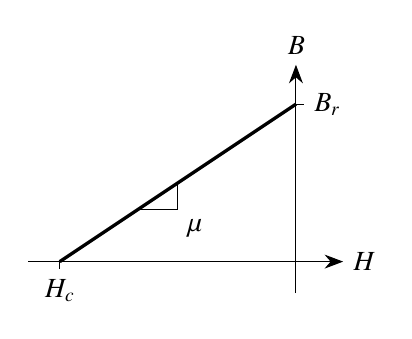
\begin{tikzpicture}
\def\scl{1.0}
\def\Br{2}
\def\Hc{-3}
% axes
\draw[-{Stealth[scale=1.4]}] (-3.4,0) -- (0.6,0) node[anchor=west] {\scalebox{\scl}{$H$}};
\draw[-{Stealth[scale=1.4]}] (0,-0.4) -- (0,2.5) node[anchor=south] {\scalebox{\scl}{$B$}};
% BH line
\draw[line width=1.2pt] (\Hc,0) -- (0,\Br);
\draw[] (\Hc,0) -- (\Hc,-0.1) node[anchor=north] {\scalebox{\scl}{$H_c$}};
\draw[] (0,\Br) -- (0.1,\Br) node[anchor=west] {\scalebox{\scl}{$B_r$}};
% mu
\draw[] (-2,0.666) -- (-1.5,0.666) node[anchor=north west] {\scalebox{\scl}{$\mu$}} -- (-1.5,1);
\end{tikzpicture}
\end{center}





%------------------------------------------------------------------------------
\clearpage
\section{Electrokinetics -- Scalar potential}
\label{sec_ksp}
%------------------------------------------------------------------------------

\hypertarget{sec_ksp}{It} is assumed that the $\sigma\vect{v}\times\vect{B}$ term can be neglected in the current density (only $\sigma\vect{E}$ remains).

\begin{table}[h!]
\centering
\begin{tabular}{lll}
\hline
\multicolumn{3}{c}{Governing law:} \\
\multicolumn{3}{c}{$\nab\cdot\vect{J}=0$}\\
$\vect{J}$ & $[\text{A}\cdot \text{m}^{-2}]$ & Current density\\
\hline

\multicolumn{3}{c}{Constitutive relation:} \\
\multicolumn{3}{c}{ $\vect{J}=\sigma\vect{E}$}\\
$\sigma$ & $[\Omega^{-1} \cdot \text{m}^{-1}]$ & Electric conductivity of medium (inverse of resistivity)\\ %\multirow{2}{*}{}
$\vect{E}=-\nab V$ & $[\text{V}\cdot \text{m}^{-1}]$ & Electric field\\
$V$ & $[\text{V}]$ & Electric potential\\
\hline

\multicolumn{3}{c}{Strong form:} \\
\multicolumn{3}{c}{$\nab\cdot\left(\sigma\nab V\right)=0$}\\
\hline

\multicolumn{3}{c}{Weak form:} \\[1pt]
\multicolumn{3}{c}{$\displaystyle\int_\Omega\sigma\nab V\cdot\nab W\,d\Omega+
\int_{\Gamma_N}\vect{n}\cdot\vect{J}\,W\,d{\Gamma_N}=0$}\\[8pt]
$V=V_D$ & \multicolumn{2}{l}{on $\Gamma_D$, constant Dirichlet (normal $\vect{J}$ and $\vect{E}$); current $I$ $[\text{A}]$ is the associated}\\
 & \multicolumn{2}{l}{(dual) global quantity for a floating potential}\\
$V=V_D(\vect{r})$ & \multicolumn{2}{l}{on $\Gamma_D$, nonhomogeneous Dirichlet (general case)}\\
$\vect{n}\cdot\vect{J}=0$ & \multicolumn{2}{l}{on $\Gamma_N$, homogeneous Neumann (tangent $\vect{J}$ and $\vect{E}$)}\\
$\vect{n}\cdot\vect{J}=J_{n,N}(\vect{r})$ & \multicolumn{2}{l}{on $\Gamma_N$, nonhomogeneous Neumann (normal component of current density)}\\
 & \multicolumn{2}{l}{(positive when current exits $\Omega$, negative when current enters $\Omega$)}\\
 
\hline
\multicolumn{3}{c}{Post-processing:} \\
$P=\int\sigma E^2\,d\Omega$ & $[\text{W}]$ & Power loss (absorbed power, Joule loss)\\[1pt]

 
\hline
\end{tabular}
\end{table}

The correspondance between the electrostatic scalar formulation (without free charges or permanent polarization) and the electrokinetic scalar formulation is  
\begin{equation}
\vect{D}\leftrightarrow\vect{J}\qquad\quad
\varepsilon_0\leftrightarrow\sigma
\end{equation}





%------------------------------------------------------------------------------
\clearpage
\section{Thermal conduction -- Scalar potential}
\label{sec_tsp}
%------------------------------------------------------------------------------

\hypertarget{sec_tsp}{The} notation used below is a mix of those found in the \textit{FEMM} software user manual and in the textbook ``\textit{A first course in finite elements}'' by Fish and Belytschko. %p.139-140

\begin{table}[h!]
\centering
\begin{tabular}{lll}
\hline
\multicolumn{3}{c}{Governing law:} \\
\multicolumn{3}{c}{$\nab\cdot\vect{q}=s$}\\
$\vect{q}$ & $[\text{W}\cdot \text{m}^{-2}]$ & Heat flux density\\
$s$ & $[\text{W}\cdot \text{m}^{-3}]$ & Volumetric heat source density\\
\hline

\multicolumn{3}{c}{Constitutive relation:} \\
\multicolumn{3}{c}{ $\vect{q}=k\vect{G}$}\\
$k$ & $[\text{W}\cdot \text{m}^{-1} \cdot \text{K}^{-1}]$ & Thermal conductivity (sometimes denoted using $\lambda$)\\ %\multirow{2}{*}{}
$\vect{G}=-\nab T$ & $[\text{K}\cdot \text{m}^{-1}]$ & Negated temperature gradient\\
$T$ & $[\text{K}]$ & Temperature (can be $[^\circ\text{C}]$ when no radiation boundary)\\
\hline

\multicolumn{3}{c}{Strong form:} \\
\multicolumn{3}{c}{$-\nab\cdot\left(k\nab T\right)=s$}\\
\hline

\multicolumn{3}{c}{Weak form:} \\[1pt]
\multicolumn{3}{c}{$\displaystyle\int_\Omega k\nab T\cdot\nab W\,d\Omega+
\int_{\Gamma_N}\vect{n}\cdot\vect{q}\,W\,d{\Gamma_N}-
\int_\Omega s\,W\,d\Omega=0$}\\[8pt]
 $T=T_D$ & \multicolumn{2}{l}{on $\Gamma_D$, constant Dirichlet (normal $\vect{q}$ and $\vect{G}$); heat flux $Q$ $[\text{W}]$ is the associated}\\
 & \multicolumn{2}{l}{(dual) global quantity for a floating temperature}\\
 $T=T_D(\vect{r})$ & \multicolumn{2}{l}{on $\Gamma_D$, nonhomogeneous Dirichlet (general case)}\\
$\vect{n}\cdot\vect{q}=0$ & \multicolumn{2}{l}{on $\Gamma_N$, homogeneous Neumann (tangent $\vect{q}$ and $\vect{G}$)}\\
$\vect{n}\cdot\vect{q}=q_{n,N}(\vect{r})$ & \multicolumn{2}{l}{on $\Gamma_N$, nonhomogeneous Neumann (normal component of heat flux density)}\\
 & \multicolumn{2}{l}{(positive when heat exits $\Omega$, negative when heat enters $\Omega$)}\\
$\vect{n}\cdot\vect{q}=(T-T_{\!0})h$ & \multicolumn{2}{l}{on $\Gamma_N$, convection boundary with heat transfer coefficient $h$ $[\text{W}\cdot \text{m}^{-2} \cdot \text{K}^{-1}]$}\\
$\vect{n}\cdot\vect{q}=(T^4-T_{\!0}^4)\beta\sigma_{\!sb}$ & \multicolumn{2}{l}{on $\Gamma_N$, radiation boundary with emissivity factor $\beta$ (generally $0\leq\beta\leq1$)}\\
 & \multicolumn{2}{l}{and the Stefan Boltzmann constant $\sigma_{\!sb}$}\\
%$\vect{F}\cdot\vect{n}=mkT/R$ & \multicolumn{2}{l}{on $\Gamma_N$, first order asymptotic boundary condition ($m$ is harmonic \#)}\\

\hline
\multicolumn{3}{c}{Post-processing:} \\
$\dot{S}_{\!p}=\int k{G^2}/{T^2}\,d\Omega$ & $[\text{W}\cdot\text{K}^{-1}]$ & Entropy production rate (assumes $T>0$)\\[1pt]

\hline
\end{tabular}
\end{table}

The correspondance between the electrostatic scalar formulation (without permanent polarization) and the themal conduction scalar formulation is  
\begin{equation}
V\leftrightarrow T\qquad\quad
\varepsilon_0\leftrightarrow k \qquad\quad
\rho\leftrightarrow s\qquad\quad
\vect{E}\leftrightarrow\vect{G}\qquad\quad
\vect{D}\leftrightarrow\vect{q}\qquad\quad
\end{equation}





%------------------------------------------------------------------------------
\clearpage
\section{Potential flow -- Scalar potential}
\label{sec_fsp}
%------------------------------------------------------------------------------

\hypertarget{sec_fsp}{An} inviscid, incompressible, irrotational fluid flow. Although the mass density is constant and has no effect on the main equations, the local conservation of mass is used as the governing law instead of the incompressibility condition $\nab\cdot \vect{v}=0$.

\begin{table}[h!]
\centering
\begin{tabular}{lll}
\hline
\multicolumn{3}{c}{Governing law:} \\
\multicolumn{3}{c}{$\nab\cdot\vect{g}=0$}\\
$\vect{g}=\rho \vect{v}$ & $[\text{kg}\cdot \text{m}^{-2}\cdot\text{s}^{-1}]$ & Momentum density\\
$\vect{v}=-\nab \varphi$ & $[\text{m}\cdot \text{s}^{-1}]$ & Velocity\\
$\varphi$ & $[\text{m}^{2}\cdot \text{s}^{-1}]$ & Velocity potential\\
$\rho$ & $[\text{kg}\cdot \text{m}^{-3}]$ & Mass density\\
\hline

\multicolumn{3}{c}{Strong form:} \\
\multicolumn{3}{c}{$\nab\cdot\left(\rho\nab \varphi\right)=0$}\\

\hline

\multicolumn{3}{c}{Weak form 1:} \\[1pt]
\multicolumn{3}{c}{$\displaystyle\int_\Omega \rho \nab \varphi\cdot\nab W\,d\Omega+
\int_{\Gamma_N}\vect{n}\cdot\vect{g}\,W\,d{\Gamma_N}=0$}\\[8pt]
  $\varphi=\varphi_D$ & \multicolumn{2}{l}{on $\Gamma_D$, constant Dirichlet (normal $\vect{g}$ and $\vect{v}$); mass flow rate $\dot{m}$ $[\text{kg}\cdot \text{s}^{-1}]$ is the}\\
 & \multicolumn{2}{l}{associated (dual) global quantity for a floating potential}\\
$\vect{n}\cdot\vect{g}=0$ & \multicolumn{2}{l}{on $\Gamma_N$, homogeneous Neumann (tangent $\vect{g}$ or $\vect{v}$)}\\
$\vect{n}\cdot\vect{g}=g_{n,N}(\vect{r})$ & \multicolumn{2}{l}{on $\Gamma_N$, nonhomogeneous Neumann (normal component of momentum density,}\\
 & \multicolumn{2}{l}{positive when flow exits $\Omega$, negative when flow enters $\Omega$)}\\
 
 \hline

\multicolumn{3}{c}{Weak form 2:} \\[1pt]
\multicolumn{3}{c}{$\displaystyle\int_\Omega \nab \varphi\cdot\nab W\,d\Omega+
\int_{\Gamma_N}\vect{n}\cdot\vect{v}\,W\,d{\Gamma_N}=0$}\\[8pt]
  $\varphi=\varphi_D$ & \multicolumn{2}{l}{on $\Gamma_D$, constant Dirichlet (normal $\vect{g}$ and $\vect{v}$); volumetric flow rate $Q$ $[\text{m}^{3}\cdot \text{s}^{-1}]$}\\
 & \multicolumn{2}{l}{is the associated (dual) global quantity for a floating potential}\\
$\vect{n}\cdot\vect{v}=0$ & \multicolumn{2}{l}{on $\Gamma_N$, homogeneous Neumann (tangent $\vect{g}$ or $\vect{v}$)}\\
$\vect{n}\cdot\vect{v}=v_{n,N}(\vect{r})$ & \multicolumn{2}{l}{on $\Gamma_N$, nonhomogeneous Neumann (normal component of velocity field,}\\
 & \multicolumn{2}{l}{positive when flow exits $\Omega$, negative when flow enters $\Omega$)}\\
 
 \hline
 \multicolumn{3}{c}{Post-processing:} \\
 $K=\frac{1}{2}\!\int\rho v^2\,d\Omega$ & $[\text{J}]$ & Kinetic energy\\[1pt]
  $q=\frac{1}{2}\,\rho v^2$ & $[\text{Pa}%=\text{J}\cdot \text{m}^{-3}=\text{kg}\cdot \text{m}^{-1}\cdot\text{s}^{-2}
  ]$ & Dynamic pressure (static pressure: $p=C-q$, where $C$ is the\\
 & & constant in Bernoulli's equation)\\
%$\vect{F}\cdot\vect{n}=mkT/R$ & \multicolumn{2}{l}{on $\Gamma_N$, first order asymptotic boundary condition ($m$ is harmonic \#)}\\
\hline
\end{tabular}
\end{table}

The correspondance between the electrostatic scalar formulation (without free charges or permanent polarization) and the potential flow scalar formulation is  
\begin{equation}
V\leftrightarrow \varphi\qquad\quad
\varepsilon_0\leftrightarrow \rho \qquad\quad
\vect{E}\leftrightarrow\vect{v}\qquad\quad
\vect{D}\leftrightarrow\vect{g}\qquad\quad
\end{equation}





%------------------------------------------------------------------------------
\clearpage
\section{Magnetoquasistatics -- Vector and scalar potentials}
\label{sec_mqs}
%------------------------------------------------------------------------------

\hypertarget{sec_mqs}{This} formulation applies when the fields are not time-invariant, but the time derivative of the electric displacement field~$\vect{D}$ is negligible compared to the free current density $\vect{J}$ in the Maxwell-Ampère law. This is a mixed formulation based on time-harmonic (phasor) extensions of the \hyperlink{sec_ksp}{Electrokinetics} and \hyperlink{sec_mvp}{Magnetostatics} formulations. Permanent magnetization is omitted. Test functions $\tilde{W}$ and $\vecp{W}$ are assumed to be separate functions (i.e. the first is not the norm of the second). 
The domain $\Omega_c$ is the nonempty conducting subdomain of $\Omega$ where Eddy currents are present, the domain $\Omega_s$ is the possibly empty subdomain of~$\Omega$ where an imposed current density $\vecp{J}_s$ exists (no Eddy-currents), % TODO: see if we can have Js in Omega_c to compute what FEMM and Agros do?
such that $\Omega_c \cap \Omega_s=0$ and $\{\Omega_c \cup \Omega_s\} \subseteq\Omega$. Example use cases:
\begin{enumerate}
\item Skin effect: voltage/current sources are related to $\Omega_c$, and $\Omega_s$ is empty ($\vecp{J}_s$ is unused);
\item Induction heating: $\Omega_s$ is nonempty and contains a known current source $\vecp{J}_s$ where induction effects are neglected (stranded conductors); no sources via voltage/current related to $\Omega_c$, where induction occurs.
\end{enumerate}

\begin{table}[h!]
\centering
\begin{tabular}{lll}
\hline
\multicolumn{3}{c}{Governing laws:} \\
\multicolumn{3}{c}{$\nab\cdot\vecp{J}=0$}\\%\qquad\qquad$\nab\times\vecp{H}=\vecp{J}$}\\
\multicolumn{3}{c}{$\nab\times\vecp{H}=\vecp{J}$}\\
\hline

\multicolumn{3}{c}{Constitutive relations:} \\
\multicolumn{3}{c}{$\vecp{J}=\sigma\vecp{E}+\vecp{J}_s$}\\%\qquad\qquad$\vecp{B}=\mu\vecp{H}$}\\
\multicolumn{3}{c}{$\vecp{B}=\mu\vecp{H}$}\\
$\vecp{E}=-\nab \tilde{V}-i\omega\vecp{A}$ & $[\text{V}\cdot \text{m}^{-1}]$ & Electric field ($i$ is the imaginary unit), in $\Omega_c$\\
$\tilde{V}$,~$\,\vecp{A}$ & $[\text{V},~\text{T}\cdot \text{m}]$ & Scalar and vector potentials, in $\Omega_c$ and $\Omega$ respectively\\
$\omega$ & $[\text{s}^{-1}]$ & Angular frequency, where $\omega=2\pi f$ and $f$ is the frequency in Hz\\
$\vecp{J}_s$ & $[\text{A}\cdot \text{m}^{-2}]$ & Imposed source current density, in $\Omega_s$, where $\nab\cdot\vecp{J}_s=0$ assumed\\
$\vecp{B}=\nab \times\vecp{A}$ & $[\text{T}]$ & Magnetic field, in $\Omega$\\
\hline

\multicolumn{3}{c}{Strong forms:} \\[1pt]
\multicolumn{3}{c}{$\nab\cdot\left(\sigma\nab \tilde{V}\right)+\nab\cdot\left(i\omega\sigma\vecp{A}\right)=0$}\\
\multicolumn{3}{c}{$\displaystyle\nab\times\left(\frac{1}{\mu}\nab\times \vecp{A}\right)=-\sigma\nab \tilde{V}-i\omega\sigma\vecp{A}+\vecp{J}_s$}\\[7pt]
\hline

\multicolumn{3}{c}{Weak forms:} \\[1pt]
\multicolumn{3}{c}{$\displaystyle
\int_{\Omega_c}\sigma\nab \tilde{V}\cdot\nab \tilde{W}\,d\Omega_c
+\int_{\Omega_c} i\omega\sigma\vecp{A}\cdot\nab \tilde{W}\,d\Omega_c
+\int_{\Gamma_{Nc}}\vect{n}\cdot\vecp{J}\,\tilde{W}\,d{\Gamma_{N_c}}=0$}\\[8pt]
\multicolumn{3}{c}{$\displaystyle
\int_\Omega\left(\frac{1}{\mu}\nab\times\vecp{A}\right)\cdot(\nab\times\vecp{W})\,d\Omega
+\int_{\Omega_c}\sigma\nab \tilde{V}\cdot\vecp{W}\,d\Omega_c
+\int_{\Omega_c} i\omega\sigma\vecp{A}\cdot\vecp{W}\,d\Omega_c$}\hspace{4cm}\\
\multicolumn{3}{c}{\hspace{7.5cm}$\displaystyle
-\int_{\Omega_s}\vecp{J}_s\cdot\vecp{W}\,d\Omega_s
+\int_{\Gamma_N}(\vect{n}\times\vecp{H})\cdot\vecp{W}\,d{\Gamma_N}=0$}\\[9pt]
$\tilde{V}=\tilde{V}_D$ & \multicolumn{2}{l}{on $\Gamma_{D_c}$, constant Dirichlet electrode potential; current $\tilde{I}$ $[\text{A}]$ is the (dual) global}\\
 & \multicolumn{2}{l}{quantity (normal $\vecp{J}$; normal $\vecp{E}$ when normal $\vecp{A}$)}\\
$\vect{n}\cdot\vecp{J}=0$ & \multicolumn{2}{l}{on $\Gamma_{N_c}$, homogeneous Neumann (tangent $\vecp{J}$; tangent $\vecp{E}$ when tangent $\vecp{A}$)}\\
%$\vect{n}\cdot\vecp{J}=\tilde{J}_{n,Nc}(\vect{r})$ & \multicolumn{2}{l}{on $\Gamma_{N_c}$, nonhomogeneous Neumann (normal component of current density)}\\
$\vect{n}\times\vecp{A}=\vect{0}$~~(or $\vecp{A}=\vect{0}$) & \multicolumn{2}{l}{on $\Gamma_D$, homogeneous Dirichlet (tangent $\vecp{H}$ and $\vecp{B}$)}\\
$\vect{n}\times\vecp{H}=\vect{0}$ & \multicolumn{2}{l}{on $\Gamma_N$, homogeneous Neumann (normal $\vecp{H}$ and $\vecp{B}$)}\\
$\vect{n}\times\vecp{H}=\vecp{A}_t/(\mu_0 R)$ & \multicolumn{2}{l}{on $\Gamma_N$, first order asymptotic boundary ($\vecp{A}_t$ is tangential component)}\\

\hline
\multicolumn{3}{c}{Post-processing:} \\
$P_c=\frac{1}{2}\int\sigma \vecp{E}\cdot\vecp{E}^*\,d\Omega_c$ & $[\text{J}]$ & Active (average) power, where $^*$ denotes the complex conjugate\\[1pt]

\hline
\end{tabular}
\end{table}



\appendix



%------------------------------------------------------------------------------
\clearpage
\section{Function spaces and symmetries in GetDP}
\label{sec_getdp}
%------------------------------------------------------------------------------

The formulations presented in this document can be applied to 2D planar (called simply 2D), 2D axisymmetric (called simply Axi or axisymmetric) or 3D domains by use of the proper function spaces and Jacobians in GetDP. Weak formulations require very little modifications when specified in the \keyw{Formulation} object in GetDP. The two main changes are: 1) the test functions appearing in the \keyw{Integral} terms (in the second argument of the inner product) use the same symbol as the unknown variable, and 2) vector source quantities should have components consisent with the chosen symmetry in 2D. For example, in a 2D simulation specified in the $x$,$y$ plane in Gmsh (at $z=0$), a current density should have a $z$ component only, while permanent magnetization/polarization should have $x$,$y$ components only. In axisymmetric simulations, the symmetry axis is the $y$ axis by default; as such, the $x$,$y$ axes represent the $r$,$z$ axes typically used when describing Axi simulations.

In the table below, the ``FS-Type'' column shows the type of function space to declare for different types of potentials. The ``Function/EntityType'' column describes the first order basis functions that are minimally required. The ``2nd order'' column shows the additional basis functions needed to support second order interpolation\footnote{In the case of edge elements, the designation of interpolation order is more intricate (and actually different) than described here. In this work, it is assumed that a vector potential is being solved, and that the order designation follows that of the geometrical elements (i.e., that second order interpolation basis functions are said to be related to second order geometrical elements for the sake of simplicity).}, assuming that second order geometrical meshing was specified in the \texttt{.geo} file using:
\begin{center}
\keyw{Mesh.HighOrderOptimize = 2;~~Mesh.ElementOrder = 2;}
\end{center}
In the ``2nd order'' column, ``None'' means that no additional basis functions need to be explicitely added since they are automatically added when second order geometrical elements are used. It is possible to use second order interpolation on first order geometrical elements, but this is not covered here.

 

\begin{table}[h!]
\centering
\begin{tabular}{llll}
\multicolumn{4}{c}{Function spaces and basis functions for scalar potentials} \\
\hline
 & FS-Type & Function / EntityType & 2nd order \\\hline
2D & \keyw{Form0} & \keyw{BF\_Node} / \keyw{NodesOf} & None (automatic)  \\
Axi & \keyw{Form0} & \keyw{BF\_Node} / \keyw{NodesOf} & None (automatic) \\
3D & \keyw{Form0} & \keyw{BF\_Node} / \keyw{NodesOf} & None (automatic) \\
 \hline
 &&&\\

 \multicolumn{4}{c}{Function spaces and basis functions for vector potentials} \\ 
 \hline
 & FS-Type & Function / EntityType &  2nd order \\\hline
2D & \keyw{Form1P} & \keyw{BF\_PerpendicularEdge} / \keyw{NodesOf} & None (automatic)  \\
Axi & \keyw{Form1P} & \keyw{BF\_PerpendicularEdge} / \keyw{NodesOf} & None (automatic) \\
3D & \keyw{Form1} & \keyw{BF\_Edge} / \keyw{EdgesOf} & \keyw{BF\_Edge\_3F\_a} / \keyw{FacetsOf} \\
 & & & \keyw{BF\_Edge\_3F\_b} / \keyw{FacetsOf} \\ 
\hline
\end{tabular}
\end{table}


Jacobians are given in the table below for the main regions of dimension $n$ of the simulation.  %Jacobians for regions of dimension $n-1$ are given after the table. 
The external Jacobian is used in the external region of open boundary models, when applicable. Only a selected set of Jacobians are listed, others can be found in the GetDP manual. 
The \keyw{Sur} Jacobian can be applied to regions of dimension $n-1$ in the 2D and 3D simulations, while the \keyw{SurAxi} Jacobian can be applied to 1D regions in axisymmetrical simulations. It is also possible to use the \keyw{VolCylShell} Jacobian in the external region of a 2D simulation, but since it internally reverts to the \keyw{VolSphShell} Jacobian, it is more natural to use \keyw{VolSphShell} (which becomes 2D in this case).

\begin{table}
\centering
\begin{tabular}{llll}
\multicolumn{4}{c}{Jacobians for main region, and external region when open boundary} \\
\hline
 & $n$ & Jacobian & External Jacobian \\\hline
2D  & 2  & \keyw{Vol} & \keyw{VolSphShell\{}$r_b$\keyw{,}$r_e$\keyw{\}}  \\
Axi & 2  & \keyw{VolAxi} & \keyw{VolAxiSphShell\{}$r_b$\keyw{,}$r_e$\keyw{\}} \\
3D & 3  & \keyw{Vol} & \keyw{VolSphShell\{}$r_b$\keyw{,}$r_e$\keyw{\}}, \keyw{VolCylShell\{}$r_b$\keyw{,}$r_e$\keyw{\}} \\
\hline
\end{tabular}
\end{table}

The $\keyw{Sur}$, $\keyw{SurAxi}$, $\keyw{Vol}$ and $\keyw{VolAxi}$ Jacobians do not have any parameters. The first two parameters of the external Jacobians are the internal ($r_b$) and external ($r_e$) radii of the shell region. The default center point for the external Jacobians is $x=y=z=0$. The default axis for the $\keyw{VolCylShell}$ Jacobian is~$z$, while the default axis for the $\keyw{VolAxi}$ and $\keyw{VolAxiSphShell}$ Jacobians is~$y$
%https://gitlab.onelab.info/getdp/getdp/-/blob/master/src/kernel/Get_Geometry.cpp?ref_type=heads#L623





%------------------------------------------------------------------------------
\clearpage
\section{Global basis functions in GetDP}
\label{sec_global}
%------------------------------------------------------------------------------

This section presents a very short and incomplete summary of global basis functions in GetDP. For a more detailed description, see tutorial \#6 in the GetDP user manual (version 4.0.0 or higher, or the development version until released).

Certain scalar potential formulations presented in this document mention a global quantity associated with a constant Dirichlet boundary condition. These global quantities can be linked to a special type of basis function in GetDP. When this is done, two options become available when imposing a constaint on a given global region. Using the electrostatics formulation as an example, the first case consists of an imposed Dirichlet constraint on the variable itself (electrostatic potential); when the global approach is used, the associated global quantity that is automatically calculated is the total charge. Conversely, it is also possible to impose the associated global quantity (the total charge here), whereby the electric potential of the region will be automatically calculated; this corresponds to situation called ``floating potential'', since the potential is not known in advance. Another example is a Dirichlet boundary of constant temperature, where the heat flux across this boundary is the associated global quantity; imposing either one allows the automatic calculation of the other.

To implement global quantities in GetDP, the nodes $r$ of a region having a constant potential must be grouped into a separate basis function with Function/Entity keywords
\begin{center}
\keyw{BF\_GroupOfNodes} / \keyw{GroupsOfNodesOf[}$r$\keyw{]};
\end{center}
these same nodes must be excluded from the main region's basis function using 
\begin{center}
\keyw{BF\_Node} / \keyw{NodesOf[All, Not}~$r$\keyw{]}.
\end{center}

A global quantity entry must also be added in the \keyw{FunctionSpace} object, to declare variables for the alias of the main unknown variable in the equation (voltage or temperature in the examples above), using \keyw{AliasOf}, and for the quantity associated with it (total charge or heat flux here), using \keyw{AssociatedWith}. A global term must also be added in the formulation (\keyw{GlobalTerm}). 





%------------------------------------------------------------------------------
\clearpage
\section{Weak form derivation notes}
\label{sec_weak}
%------------------------------------------------------------------------------

To obtain the weak forms, these main steps are followed. 

For the scalar potential formulations:
\begin{enumerate}
\item Multiply the governing law by the test function $W$ and integrate over $\Omega$;
\item Apply the vector identity $W(\nab\cdot\vect{F})=\nab\cdot(W\vect{F})-\vect{F}\cdot(\nab W)$ to the divergence term;
\item Invoke the divergence theorem $\int\nab\cdot(W\vect{F})\,d\Omega=\int(W\vect{F})\cdot\vect{n}\,d\Gamma$ on the first of the two resulting terms of the previous indentity, and rearrange to obtain an integrand of the form $(\vect{n}\cdot\vect{F})\,W$;
\item Substitute any constitutive laws as required.
\end{enumerate}


For the vector potential formulations:
\begin{enumerate}
\item Perform a dot product of the governing law and the test function $\vect{W}$ and integrate over $\Omega$;
\item Apply the vector identity $\vect{W}\cdot(\nab\times\vect{F})=\nab\cdot(\vect{F}\times\vect{W})+\vect{F}\cdot(\nab\times\vect{W})$ to the curl term;
\item Invoke the divergence theorem $\int\nab\cdot(\vect{F}\times\vect{W})\,d\Omega=\int(\vect{F}\times\vect{W})\cdot\vect{n}\,d\Gamma$ on the first of the two resulting terms of the previous indentity, and rearrange using a tripple product identity to obtain an integrand of the form $(\vect{n}\times\vect{F})\cdot\vect{W}$;
\item Substitute any constitutive laws as required.
\end{enumerate}




\end{document}

